\documentclass[12pt,a4paper]{article}
\usepackage{cmap} % Makes the PDF copiable. See http://tex.stackexchange.com/a/64198/25761
\usepackage[T1]{fontenc}
\usepackage[brazil]{babel}
\usepackage[utf8]{inputenc}
\usepackage{amsmath}
\usepackage{amsfonts}
\usepackage{amssymb}
\usepackage{amsthm}
\usepackage{textcomp} % \degree
\usepackage{gensymb} % \degree
\usepackage[usenames,svgnames,dvipsnames]{xcolor}
\usepackage{hyperref}
\usepackage{multicol}
\usepackage{graphicx}
\usepackage[margin=2cm]{geometry}
\usepackage{systeme}
\usepackage{icomma}

\hypersetup{
   colorlinks = true,
   allcolors = {blue}
}

% TODO: Consider using exsheets
% http://linorg.usp.br/CTAN/macros/latex/contrib/exsheets/exsheets_en.pdf
%
% http://ctan.org/tex-archive/macros/latex/contrib/exercise/
% Options: answerdelayed,lastexercise,noanswer
\usepackage[answerdelayed,lastexercise]{exercise}

\addto\captionsbrazil{%
\def\listexercisename{Lista de exerc\'icios}%
\def\ExerciseName{Exerc\'icio}%
\def\AnswerName{Solu\c{c}\~ao do exerc\'icio}%
\def\ExerciseListName{Ex.}%
\def\AnswerListName{Solu\c{c}\~ao}%
\def\ExePartName{Parte}%
\def\ArticleOf{de\ }%
}

\renewcommand{\ExerciseHeaderTitle}{(\ExerciseTitle)\ }
\renewcommand{\ExerciseListHeader}{%\ExerciseHeaderDifficulty%
\textbf{%\ExerciseListName\
\ExerciseHeaderNB.\ %
%\ --- \
\ExerciseHeaderTitle}%
%\ExerciseHeaderOrigin
\ignorespaces}
\renewcommand{\AnswerListHeader}{\textbf{\ExerciseHeaderNB.\ (\AnswerListName)\ }}
\newcommand*\R{\mathbb{R}}

% Loop Space / CC BY-SA-3.0 / https://tex.stackexchange.com/a/3164/25761
%--------grstep
% For denoting a Gauss' reduction step.
% Use as: \grstep{\rho_1+\rho_3} or \grstep[2\rho_5 \\ 3\rho_6]{\rho_1+\rho_3}
\newcommand{\grstep}[2][\relax]{%
   \ensuremath{\mathrel{
       {\mathop{\longrightarrow}\limits^{#2\mathstrut}_{
                                     \begin{subarray}{l} #1 \end{subarray}}}}}}

\renewcommand{\theenumi}{\alph{enumi}}
\renewcommand\labelenumi{(\theenumi) }

\newcommand*\tipo{Prova II}
\newcommand*\turma{CCI192-04U}
\newcommand*\disciplina{ANN0001}
\newcommand*\eu{Helder G. G. de Lima}
\newcommand*\data{29/05/2024}

\author{\eu}
\title{\tipo - \disciplina}
\date{\data}

\begin{document}
\thispagestyle{empty}
\newgeometry{margin=2cm,bottom=0.5cm}
\begin{center}

\includegraphics[width=9.0cm]{marca} \\
\textbf{\tipo\ (\disciplina / \turma)} \\
Prof. \eu\footnote{
Este é um material de acesso livre distribuído sob os termos da licença \href{https://creativecommons.org/licenses/by-sa/4.0/deed.pt_BR}{Creative Commons BY-SA 4.0}}
\end{center}

\noindent Nome do(a) aluno(a): \underline{\hspace{9,7cm}} Data: \underline{\data}

%\section*{Instruções}
\begin{center}\fbox{
\begin{minipage}{14cm}
\begin{footnotesize}
\begin{itemize}
\renewcommand{\theenumi}{\Roman{enumi}}
\item Identifique-se em todas as folhas.
\item Mantenha o celular e os demais equipamentos eletrônicos desligados durante a prova.
\item Justifique cada resposta com cálculos ou argumentos baseados na teoria estudada.
\item Resolva $5$ das $6$ questões (deixe claro que questão não deverá ser corrigida).
\end{itemize}
\end{footnotesize}
\end{minipage}
}
\end{center}

%\section*{Questões}
\begin{ExerciseList}
\Exercise[title={2,0}] Um dos passos para determinar certo spline cúbico natural interpolador é resolver:
\[
  \begin{bmatrix}
    2 & 1 & 0 \\
    10 & 40 & 10 \\
    0 & 1 & 2\\
  \end{bmatrix}
  \cdot
  \begin{bmatrix}
    y_0^\prime\\
    y_1^\prime\\
    y_2^\prime\\
  \end{bmatrix}
  =
  \begin{bmatrix}
    6\\
    0\\
    -6\\
  \end{bmatrix}.
\]
Dê evidências teóricas de que as soluções $y_i^\prime$ podem ser obtidas pelo método de Gauss-Seidel, e calcule-as com estimativa de erro absoluto menor que $0,1$, considerando $(3, -1,-4)$ como aproximação inicial.
{\color{blue} \textit{(Arredonde os valores obtidos com 2 algarismos após a vírgula)}}

\Answer Considerando que
$|2| > |1|+|0|$,
$|40| > |10|+|10|$ e
$|2| > |0|+|1|$
a matriz de coeficientes é estritamente diagonalmente dominante, e portanto a sequência gerada pelo método de Gauss-Seidel convergirá, qualquer que seja a aproximação inicial escolhida. Denotando a aproximação obtida na $k$-ésima iteração por $\left(y_0^{(k)}, y_1^{(k)}, y_2^{(k)}\right)$, essa aproximação é dada por:
\[
  \begin{cases}
    y_0^{(k)} = \left(6 - y_1^{(k-1)}\right)/2, \\
    y_1^{(k)} = \left(- 10 y_0^{(k)} - 10y_2^{(k-1)}\right)/40, \\
    y_2^{(k)} = \left(-6 - y_1^{(k)}\right)/2.
    \end{cases}
\]
Os valores obtidos a cada iteração são os seguintes:
\medskip
\begin{center}
\begin{tabular}{crrrrr}
\hline
$\boldsymbol{k}$     & 0 & 1 & 2 & 3\\
\hline
$\boldsymbol{y_0^{(k)}}$ &  3,00 &  3,50 &  2,94 &  2,99 \\
$\boldsymbol{y_1^{(k)}}$ & -1,00 &  0,13 &  0,03 &  0,01 \\
$\boldsymbol{y_2^{(k)}}$ & -4,00 & -3,07 & -3,02 & -3,01 \\
\hline
$\varepsilon_{abs}$ & - & 1,13 & 0,56 & 0,05\\
\hline
\end{tabular}
\end{center}


\Exercise[title={2,0}] Sabendo que o spline cúbico natural $s(x)$ associado à equação da questão anterior interpola os pontos $(-8, 0)$, $(2, 20)$ e $(12, 0)$, e lembrando que a solução exata $(y_0^\prime, y_1^\prime, y_2^\prime) = (3, 0, -3)$ consiste das derivadas do spline cúbico natural $s(x)$ nesses pontos, escreva $s(x)$ explicitamente.
\Answer Considerando os pontos dados, o spline tem a forma
\[
  s(x) =
  \begin{cases}
    a_0 + b_0(x + 8) + c_0(x + 8)^2 +d_0(x + 8)^3, & \text{ se } -8 \leq x \leq 2,\\
    a_1 + b_1(x - 2) + c_1(x - 2)^2 +d_1(x - 2)^3, & \text{ se } 2 \leq x \leq 12,
  \end{cases}
\]
Os valores de $a_i$, $b_i$, $c_i$ e $d_i$, para $i \in \{1, 2\}$ podem ser determinados de duas maneiras:

\textbf{Alternativa 1}: Usando os valores conhecidos de $y'_0$, $y'_1$ e $y'_2$ e considerando $h_0 = x_1 - x_0 = 2 - (-8) = 10$, $h_1 = x_2 - x_1 = 12 - 2 = 10$, tem-se
\[
\begin{cases}
  a_0 & = y_0 = 0,\\
  b_0 & = y'_0 = 3,\\
  c_0 & = 3\dfrac{y_1-y_0}{h_0^2}-\dfrac{y'_1+2y'_0}{h_0}
        = 3\cdot \dfrac{20-0}{10^2}-\dfrac{0 + 2\cdot 3}{10}
        = 0,\\
  d_0 & = -2\dfrac{y_1-y_0}{h_0^3}+\dfrac{y'_1+y'_0}{h_0^2}
        = -2\cdot \dfrac{20-0}{10^3}+\dfrac{0+3}{10^2}
        = -0,01,\\
\end{cases}
\]
e
\[
\begin{cases}
  a_1 & = y_1 = 20,\\
  b_1 & = y'_1 = 0,\\
  c_1 & = 3\dfrac{y_2-y_1}{h_1^2}-\dfrac{y'_2+2y'_1}{h_1}
        = 3\cdot \dfrac{0-20}{10^2}-\dfrac{-3 + 2\cdot 0}{10}
        = -0,3,\\
  d_1 & = -2\dfrac{y_2-y_1}{h_1^3}+\dfrac{y'_2+y'_1}{h_1^2}
        = -2\cdot \dfrac{0-20}{10^3}+\dfrac{-3+0}{10^2}
        = 0,01.
\end{cases}
\]

\textbf{Alternativa 2}: Primeiramente, usando os valores conhecidos de $s$ e $s^\prime$ em $x_0 = -8$, tem-se:
\[
  \begin{cases}
    s(-8) & = 0, \\
    s^\prime(-8) & = 3
  \end{cases}
  \Rightarrow
  \begin{cases}
    a_0 + b_0(-8 + 8) + c_0(-8 + 8)^2 + d_0(-8 + 8)^3 & = 0, \\
    b_0 + 2c_0(-8 + 8) +3d_0(-8 + 8)^2 & = 3
  \end{cases}
  \Rightarrow
  \begin{cases}
    a_0 & = 0, \\
    b_0 & = 3.
  \end{cases}
\]
Consequentemente, usando os valores conhecidos de $s$ e $s^\prime$ em $x_1 = 2$, tem-se:
\[
  \begin{cases}
    s(2) & = 20, \\
    s^\prime(2) & = 0
  \end{cases}
  \Rightarrow
  \begin{cases}
    0 + 3\cdot (2 + 8) + c_0(2 + 8)^2 + d_0(2 + 8)^3 & = 20, \\
    3 + 2c_0(2 + 8) +3d_0(2 + 8)^2 & = 0
  \end{cases}
  \Rightarrow
  \begin{cases}
    10 c_0 + 100 d_0 & = -1, \\
    20 c_0 + 300 d_0 & = -3
  \end{cases}
\]
e por Cramer, conclui-se que $c_0 = 0$ e $d_0 = -\frac{1}{100}$.

Na sequência, usando os valores conhecidos de $s$ e $s^\prime$ em $x_1 = 2$, resulta que
\[
  \begin{cases}
    s(2) & = 20, \\
    s^\prime(2) & = 0
  \end{cases}
  \Rightarrow
  \begin{cases}
    a_1 + b_1(2 - 2) + c_1(2 - 2)^2 + d_1(2 - 2)^3 & = 20, \\
    b_1 + 2c_1(2 - 2) +3d_1(2 - 2)^2 & = 0
  \end{cases}
  \Rightarrow
  \begin{cases}
    a_1 & = 20, \\
    b_1 & = 0.
  \end{cases}
\]
Consequentemente, usando os valores conhecidos de $s$ e $s^\prime$ em $x_1 = 12$, tem-se:
\[
  \begin{cases}
    s(12) & = 0, \\
    s^\prime(12) & = -3
  \end{cases}
  \Rightarrow
  \begin{cases}
    20 + 0\cdot (12 - 2) + c_1(12 - 2)^2 + d_1(12 - 2)^3 & = 0, \\
    0 + 2c_1(12 - 2) +3d_1(12 - 2)^2 & = -3
  \end{cases}
  \Rightarrow
  \begin{cases}
    10 c_1 + 100 d_1 & = -2, \\
    20 c_1 + 300 d_1 & = -3.
  \end{cases}
\]
Por Cramer, obtém-se $c_1 = -\frac{3}{10}$ e $d_1 = \frac{1}{100}$.

Portanto, substituindo os valores obtidos por qualquer um dos métodos. conclui-se que
\[
  s(x) =
  \begin{cases}
    3 (x + 8) - 0,01(x + 8)^3, & \text{ se } -8 \leq x \leq 2,\\
    20 - 0,3(x - 2)^2 + 0,01(x - 2)^3, & \text{ se } 2 \leq x \leq 12.
  \end{cases}
\]


\textit{Observação}: Para fins de validação, note que, de fato, $s(-8) = 0$, $s(2) = 20$ e $s(12) = 0$. Graficamente, $s(x)$ tem a seguinte representação:

\begin{center}
  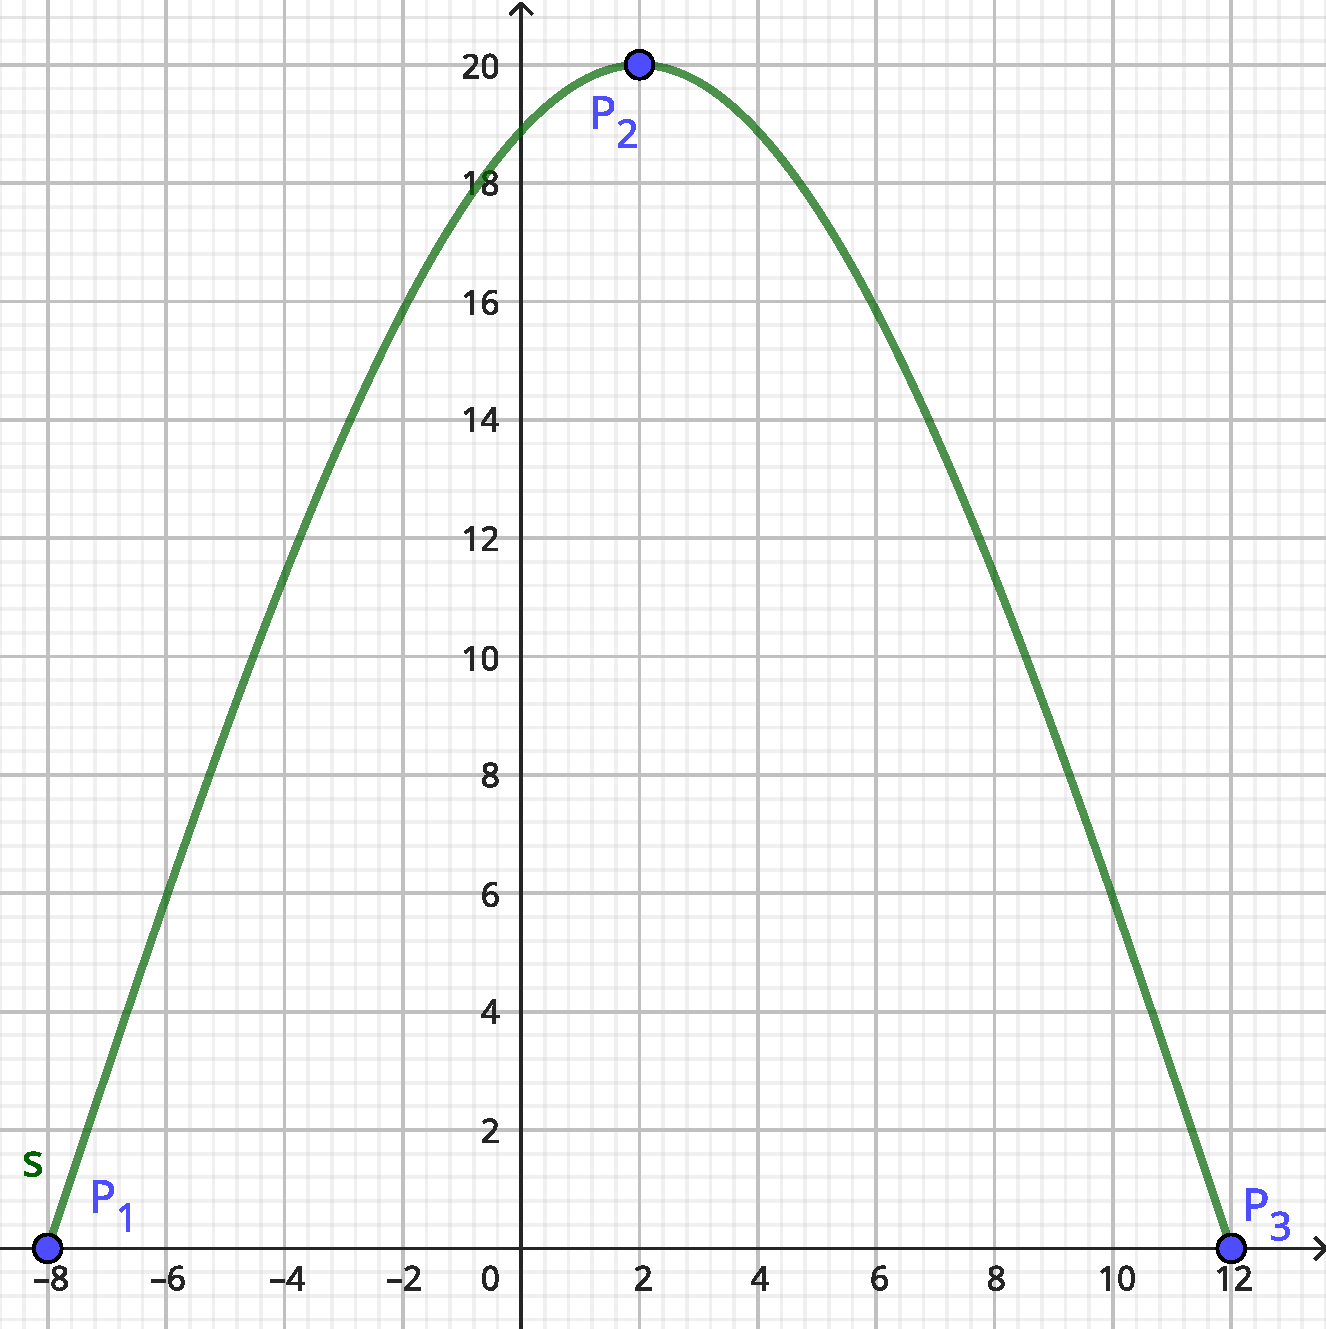
\includegraphics[width=8.0cm]{img/prova-2-cci-spline-de-ordem-3-natural.pdf}
\end{center}


\Exercise[title={2,0}] Determine os valores de $k \in \R$ para os quais todas as entradas da matriz $L$ da fatoração $LU$ de $A=\begin{bmatrix}
  2 & 3 & 4 \\
  2 & 4 & 3 \\
  6 & k & 20 -k
\end{bmatrix}$ são maiores ou iguais a zero.

\Answer Através de operações elementares, obtém-se

\[
\begin{bmatrix}
  2 & 3 & 4 \\
  2 & 4 & 3 \\
  6 & k & 20 -k
\end{bmatrix}
\grstep[L_3 \to L_3 -3 L_1]{L_2 \to L_2 - 1 L_1}
\begin{bmatrix}
  2 & 3 & 4 \\
  0 & 1 & -1 \\
  0 & k-9 & 8 -k
\end{bmatrix}
\grstep{L_3 \to L_3 -(k-9)L_2}
\begin{bmatrix}
  2 & 3 & 4 \\
  0 & 1 & -1 \\
  0 & 0 & -1
\end{bmatrix}.
\]

Então $A = LU$, em que
\[
L =
\begin{bmatrix}
1 & 0 & 0 \\
1 & 1 & 0 \\
3 & k - 9 & 1
\end{bmatrix}
\text{ e }
U =
\begin{bmatrix}
2 & 3 & 4 \\
0 & 1 & -1 \\
0 & 0 & -1
\end{bmatrix}.
\]
Assim, $L$ terá todas as entradas maiores ou iguais a zero se $k - 9 \geq 0$, ou seja, se $k \geq 9$.

\Exercise[title={2,0}] Determine (por diferenças divididas de Newton ou por Lagrange), o polinômio $p(x)$ que interpola $f(x) = x^2 - 2^x$ em $x_0 = 2$, $x_1 = 3$, $x_2 = 4$ e $x_3 = 5$ e calcule o erro absoluto da aproximação $f(7/2) \approx p(7/2)$.
{\color{blue} \textit{(Arredonde a resposta com 2 algarismos após a vírgula)}}
\Answer A partir dos pontos dados, obtém-se por diferenças divididas de Newton:
\[
\begin{array}{cccccc}
x_i
& y_i=f[x_i]
& f[x_i,x_{i+1}]
& f[x_i,x_{i+1},x_{i+2}]
& f[x_i,\ldots,x_{i+3}]\\
2 & \mathbf{0} \\
  & & \mathbf{1} \\
3 & 1 & & \mathbf{-1} \\
  & & -1 & & \mathbf{-\frac{2}{3}} \\
4 & 0 & & -3\\
  & & -7 \\
5 & -7
\end{array}
\]

Então:
\begin{align*}
p(x)
&=0
 +1 (x-2)
 -1 (x-2)(x-3)
 -\frac{2}{3} (x-2)(x-3)(x-4)
  = -\frac{2}{3}x^3 + 5x^2 - \frac{34}{3} + 8.
\end{align*}
Usando este polinômio para estimar o valor pedido, resulta que:
\begin{align*}
  p\left(\frac{7}{2}\right)
  & =\left(\frac{7}{2}-2\right)
  -\left(\frac{7}{2}-2\right)\left(\frac{7}{2}-3\right)
  -\frac{2}{3} \left(\frac{7}{2}-2\right)\left(\frac{7}{2}-3\right)\left(\frac{7}{2}-4\right) \\
  & =\frac{3}{2}
  -\frac{3}{2} \cdot \frac{1}{2}
  -\frac{2}{3} \cdot \frac{3}{2}\cdot \frac{1}{2}\cdot \frac{-1}{2}
  =\frac{3}{2}
  -\frac{3}{4}
  +\frac{1}{4}
  = 1.
\end{align*}
Então o erro absoluto é $\varepsilon_{abs} = |f(7/2) - p(7/2)| = \left|\left(\frac{7}{2}\right)^2 - 2^{\frac{7}{2}} - 1 \right| \approx |0,93629 - 1| \approx 0,06$.

\textbf{Solução 2}: Considerando que $f(2) = 0$, $f(3) = 1$ e $f(4) = 0$ e $f(5)=-7$, o método de Lagrange fornece a seguinte expressão para o polinômio que interpola $f$ nos pontos dados:
\begin{align*}
p(x)
  & = 0 L_0(x) + 1 L_1(x) + 0 L_2(x) - 7 L_3(x)
    = L_1(x) - 7 L_3(x) \\
  & = \frac{(x-2)(x-4)(x-5)}{(3-2)(3-4)(3-5)}
  -7 \frac{(x-2)(x-3)(x-4)}{(5-2)(5-3)(5-4)}\\
  & = \frac{1}{2}(x-2)(x-4)(x-5)
   -\frac{7}{6}(x-2)(x-3)(x-4)
    = -\frac{2}{3}x^3 + 5x^2 - \frac{34}{3} + 8.
\end{align*}
Logo,
\begin{align*}
  p\left(\frac{7}{2}\right)
  & = \frac{1}{2}\left(\frac{7}{2}-2\right)\left(\frac{7}{2}-4\right)\left(\frac{7}{2}-5\right)
    - \frac{7}{6}\left(\frac{7}{2}-2\right)\left(\frac{7}{2}-3\right)\left(\frac{7}{2}-4\right) \\
  & = \frac{1}{2}\cdot\frac{3}{2}\cdot\frac{-1}{2}\cdot\frac{-3}{2}
    - \frac{7}{6}\cdot\frac{3}{2}\cdot\frac{1}{2}\cdot\frac{-1}{2}
    = \frac{9}{16} + \frac{7}{16}
    = 1.
\end{align*}

Como antes, tem-se $\varepsilon_{abs} = |f(7/2) - p(7/2)| \approx 0,06$.

A figura a seguir mostra os gráficos de $f(x)$ e $p(x)$:

\begin{center}
  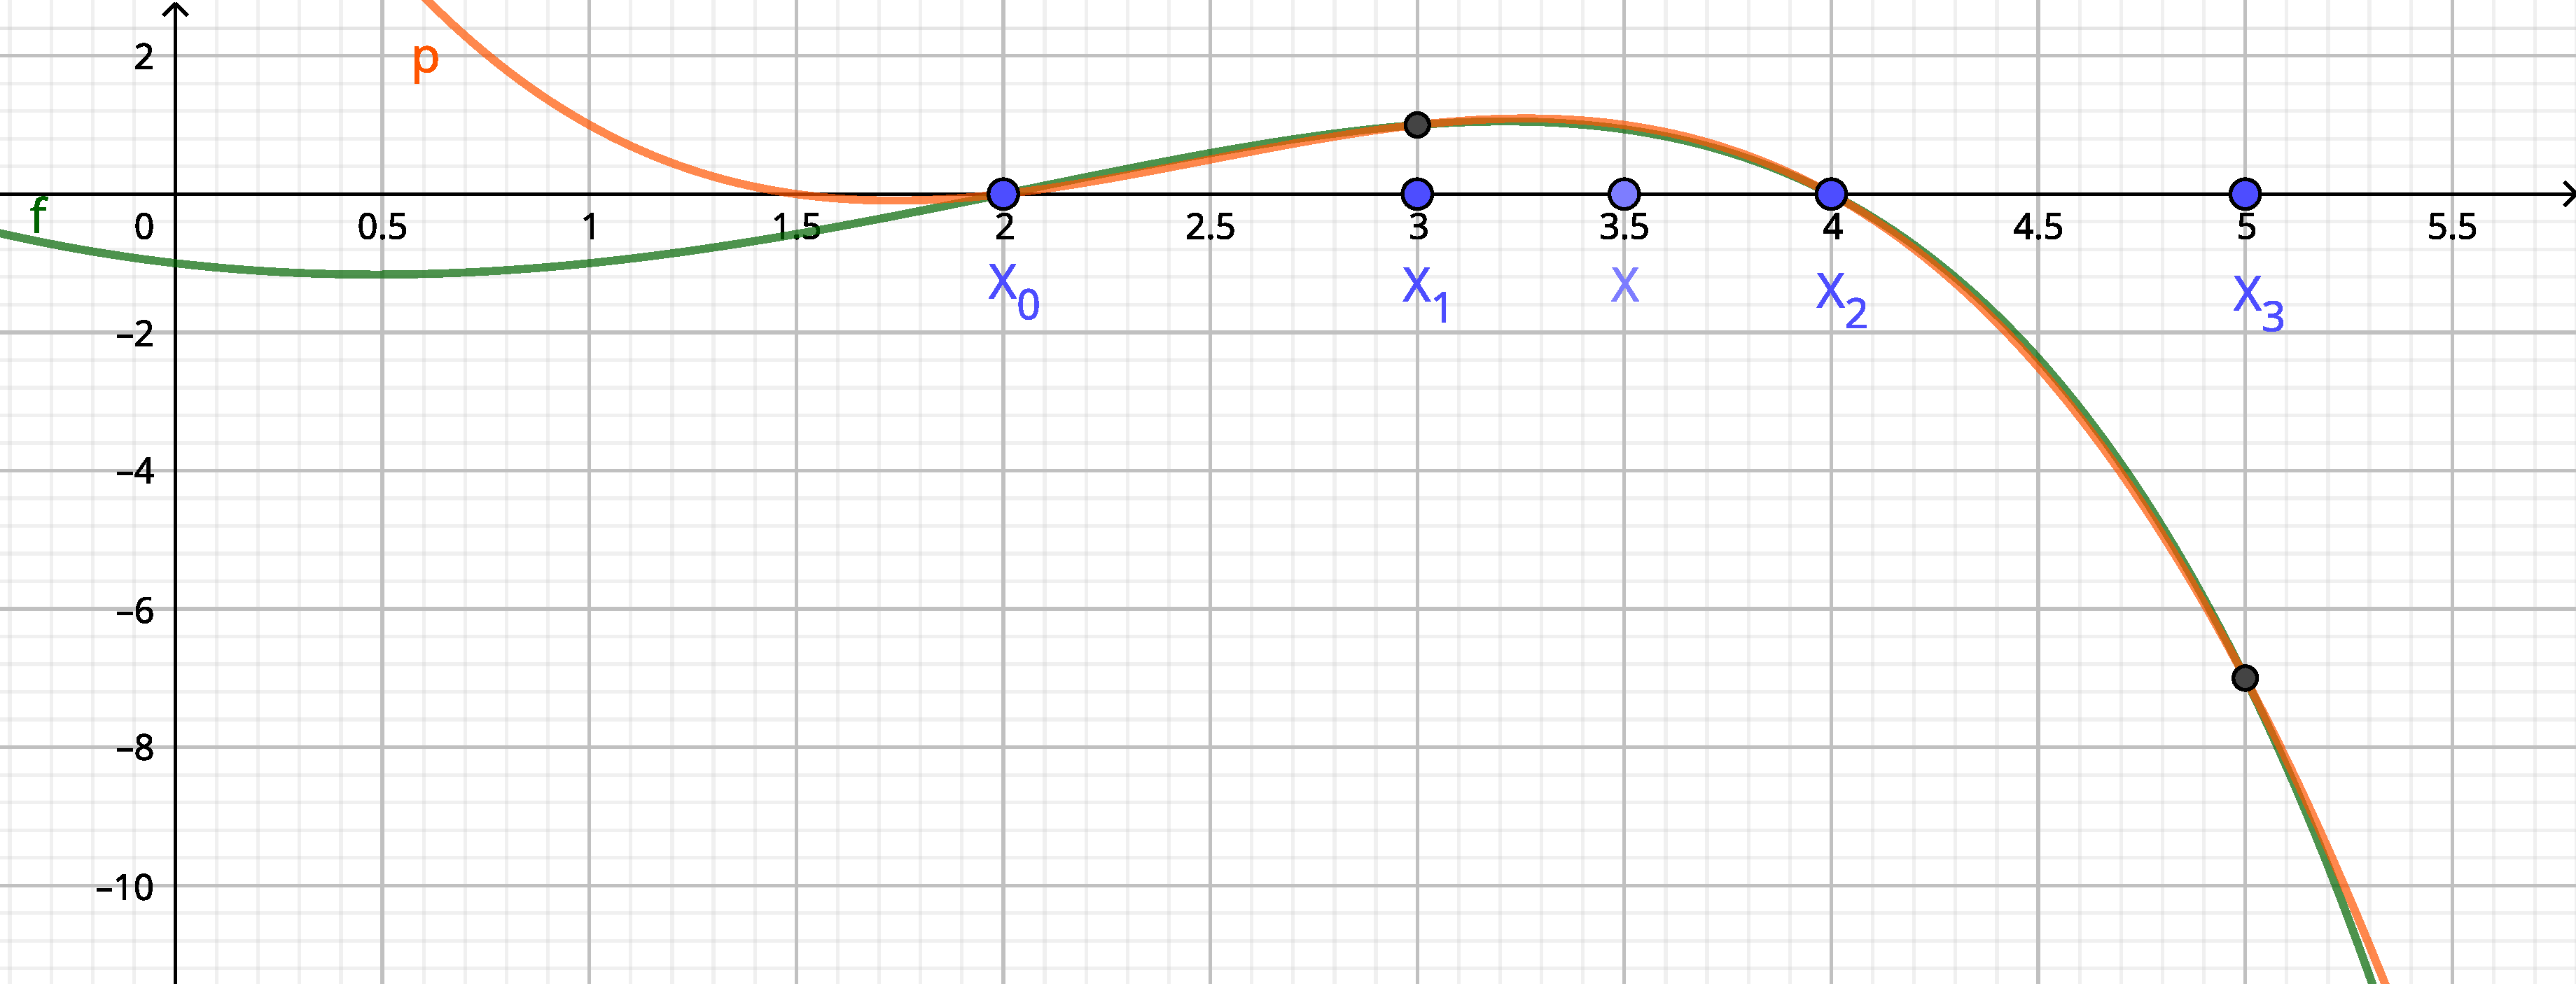
\includegraphics[width=10.0cm]{img/prova-2-cci-interpolação.pdf}
\end{center}


\Exercise[title={2,0}]
Seja $\varphi(x_1, x_2) = \left(\dfrac{{x_2}^2+1}{4}, \dfrac{{x_1}^2+1}{8}\right)$ uma função de iteração para o sistema não linear:
\[
  \begin{cases}
  4x_1-{x_2}^2 = 1\\
  {x_1}^2-8x_2 = -1.
  \end{cases}
\]
Mostre que se $X \in Q = [0, 1] \times [0,1]$, então $\varphi(X) \in Q$, e portanto $\varphi$ tem ponto fixo.
\Answer Para quaisquer $x_1$ e $x_2$ tais que $0 \leq x_1 \leq 1$ e $0 \leq x_2 \leq 1$, tem-se:
\[
  0 \leq x_2 \leq 1
  \Rightarrow
  0^2 \leq {x_2}^2 \leq 1^2
  \Rightarrow
  1 \leq {x_2}^2+1 \leq 2
  \Rightarrow
  \frac{1}{4} \leq \frac{{x_2}^2+1}{4} \leq \frac{1}{2}
  \Rightarrow
  \frac{1}{4} \leq \varphi_1(x_1, x_2) \leq \frac{1}{2}
\]
e
\[
  0 \leq x_1 \leq 1
  \Rightarrow
  0^2 \leq {x_1}^2 \leq 1^2
  \Rightarrow
  1 \leq {x_1}^2+1 \leq 2
  \Rightarrow
  \frac{1}{8} \leq \frac{{x_1}^2+1}{8} \leq \frac{1}{4}
  \Rightarrow
  \frac{1}{8} \leq \varphi_2(x_1, x_2) \leq \frac{1}{4}.
\]
Em outras palavras, $\varphi_1(x_1, x_2) \in \left[\frac{1}{4}, \frac{1}{2}\right] \subset [0, 1]$ e $\varphi_2(x_1, x_2) \in \left[\frac{1}{8}, \frac{1}{4}\right] \subset [0, 1]$. Logo, $\varphi(x_1, x_2) \in Q$ sempre que $(x_1, x_2) \in Q$, e como $\varphi_1$ e $\varphi_2$ são contínuas (por serem polinômios), $\varphi$ tem um ponto fixo em $Q$.

A figura a seguir mostra que as imagens dos pontos de $Q$ pela função de iteração $\varphi$ formam o retângulo $\left[\frac{1}{4}, \frac{1}{2}\right] \times [\frac{1}{8}, \frac{1}{4}]$ que está contido do quadrado $Q$:

\begin{center}
  \includegraphics[width=6.0cm]{img/prova-2-cci-domínio-e-imagem.pdf}
\end{center}

\Exercise[title={2,0}] Utilize $\varphi$ e a aproximação inicial $X^{(0)}=(x_1^{(0)}, x_2^{(0)}) = (\frac{3}{4}, \frac{1}{4})$ para aproximar a solução do sistema anterior por iteração de ponto fixo, com erro relativo estimado menor que $0,1$.

{\color{blue} \textit{(Arredonde os valores obtidos com 4 algarismos após a vírgula)}}
\Answer Nas primeiras iterações do método do ponto fixo, usando as relações
\[
\begin{cases}
x_1^{(k)} = \frac{\left[x_2^{(k)}\right]^2+1}{4}, \\
x_2^{(k)} = \frac{\left[x_1^{(k)}\right]^2+1}{8},
\end{cases}
\]
obtêm-se essas aproximações:
\medskip
\begin{center}
\begin{tabular}{crrrrr}
\hline
$\boldsymbol{k}$     & 0 & 1 & 2 & 3\\
\hline
$\boldsymbol{x_1^{(k)}}$ & 0,7500 & 0,2656 & 0,2595 & 0,2545 \\
$\boldsymbol{x_2^{(k)}}$ & 0,2500 & 0,1953 & 0,1338 & 0,1334 \\
\hline
$\varepsilon_{abs}$ & - & 0,4844 & 0,0615 & 0,0050 \\
$\varepsilon_{rel}$ & - & 1,8238 & 0,2370 & \textbf{0,0196} \\
\hline
\end{tabular}
\end{center}
\medskip

Portanto, a solução é aproximadamente $({x_1}^{(3)}, {x_2}^{(3)}) = (0,2545, 0,1334)$, com erro relativo estimado $0,0196 < 0,1$.

A figura a seguir mostra as curvas correspondentes a cada equação, bem como os pontos obtidos nas primeiras iterações:

\begin{center}
  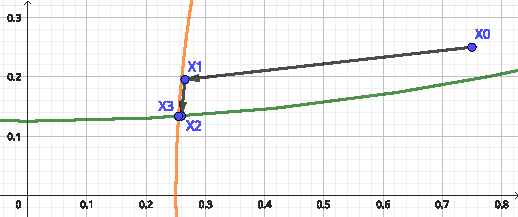
\includegraphics[width=10.0cm]{img/prova-2-cci-iterações-ponto-fixo.pdf}
\end{center}
\end{ExerciseList}

\begin{center}
BOA PROVA!
\end{center}

\newpage
\restoregeometry
\section*{Respostas}
\shipoutAnswer
\end{document}
